\documentclass{article}
\usepackage[utf8]{inputenc}
\usepackage{amsmath}
\usepackage{amssymb}
\usepackage{graphicx}
\usepackage{listings}

\begin{document}
\section*{Structured matrix-vector product}
For $n \in \mathbb{N}, n > 0$ we conside the real $n \times n$ matrix $\mathbf{A}$ defined by
\begin{equation*}
    \left(\mathbf{A}\right)_{i,j} = a_{ij} = \text{min}\left\{i,j\right\}\, , \: i,j = 1,\dots, n 
\end{equation*}
given the structure of the matrix $\mathbf{A}$ we can implement the following code which computes $\mathbf{y} = \mathbf{A}\mathbf{x}$.
\begin{figure}[!hbt]
    \centering
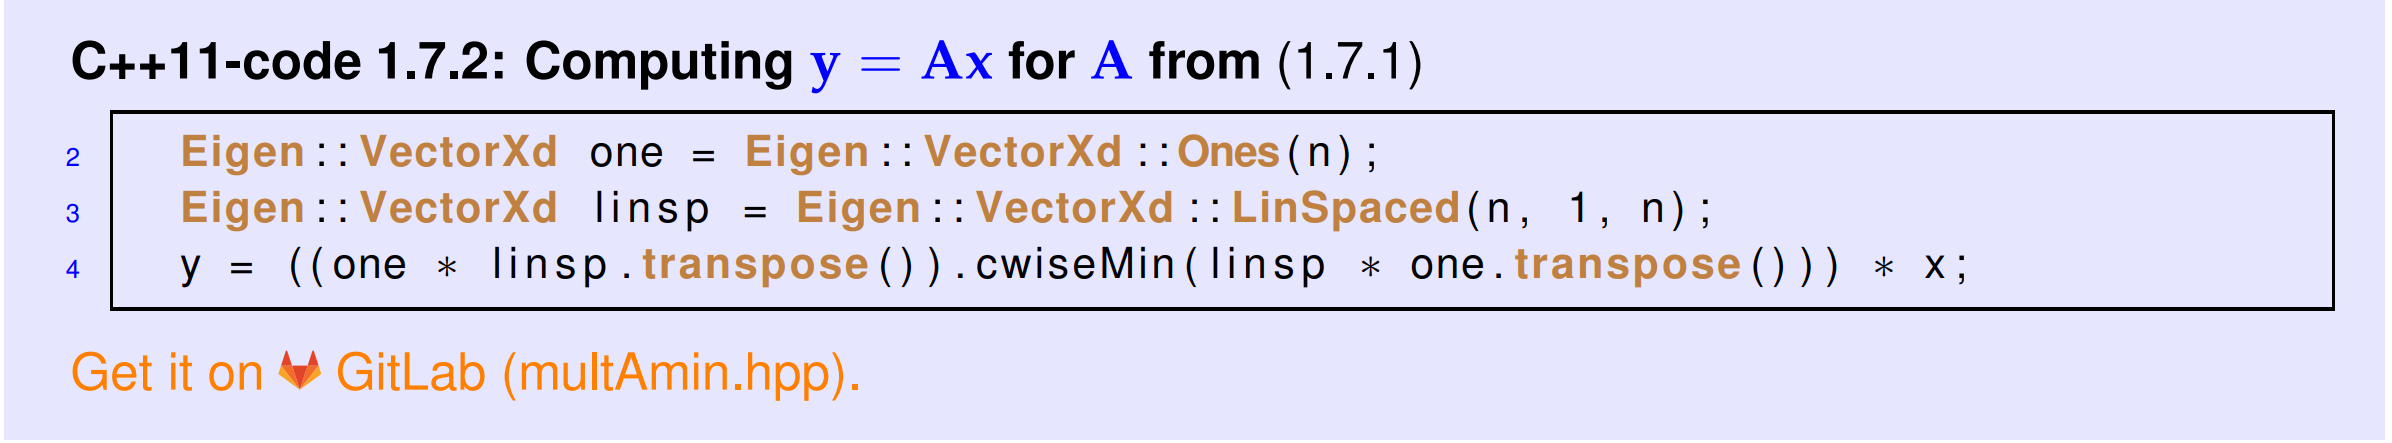
\includegraphics[width=1.0\linewidth]{1-7Code.png}
\end{figure}

\subsection*{1-7.a} We are tasked with finding the asymptotic complexity of the given \verb|C++| function. The first line takes $\mathcal{O}\left(n\right)$ operations as it constructs a vector of size $n$. The second one does also construct a vector of size $n$ and hence also takes $\mathcal{O}\left(n\right)$  operations. The third one we must observe a bit more closely. We compute the following result
\begin{equation*}
    \text{cwiseMin}\left(\begin{bmatrix}
        1 \\1\\ \vdots \\ 1
    \end{bmatrix} * \begin{bmatrix}
        1 & 2 & \dots & n
    \end{bmatrix} \: , \: \begin{bmatrix}
        1 \\2 \\ \dots \\ n
    \end{bmatrix}*
    \begin{bmatrix}
        1 & 1& \dots & 1
    \end{bmatrix}\right) * \mathbf{x}
\end{equation*}
This evaluates to
\begin{equation*}
    \text{cwiseMin}\left(
    \begin{bmatrix}
    1 & 2 & \dots & n \\
    1 & 2 & \dots & n \\
    \vdots & \vdots & & \vdots \\
    1 & 2 & \dots & n
    \end{bmatrix} \: , \: \begin{bmatrix}
     1 & 1 & \dots & 1 \\
    2 & 2 & \dots & 2 \\
    \vdots & \vdots & & \vdots \\
    n & n & \dots & n
    \end{bmatrix}
    \right) * \mathbf{x} = \begin{bmatrix}
        1 & 1 & 1 & \dots & 1 \\
        1 & 2 & 2 & \dots & 2 \\
        1 & 2 & 3 & \dots & 3 \\
        \vdots & \vdots & \vdots &\ddots & \vdots \\
        1 & 2 & 3 & \dots & n
    \end{bmatrix} * \mathbf{x}
\end{equation*}
This operation is hence in $\mathcal{O}\left(n^{2}\right)$ as both an entry-wise minimun and a matrix-vector product are computed. Overall we thus get $\mathcal{O}\left(n^{2}\right)$
\subsection*{1-7.b}
We need to observe what the product we wrote down in 1-7.a evaluates to
\begin{equation*}
   \begin{bmatrix}
        1 & 1 & 1 & \dots & 1 \\
        1 & 2 & 2 & \dots & 2 \\
        1 & 2 & 3 & \dots & 3 \\
        \vdots & \vdots & \vdots &\ddots & \vdots \\
        1 & 2 & 3 & \dots & n
    \end{bmatrix} * \begin{bmatrix}
        x_{1} \\ x_{2} \\ x_{3} \\ \vdots \\ x_{n}
    \end{bmatrix} = 
    \begin{bmatrix}
        x_{1} + x_{2} + x_{3} + \dots + x_{n} \\
        x_{1} + 2\left(x_{2} + x_{3} + \dots + x_{n}\right) \\
        x_{1} + 2x_{2} + 3\left(x_{3} + \dots + x_{n}\right) \\
        \vdots
        \\
        x_{1} + 2x_{2} + 3x_{3} + \dots + nx_{n}
    \end{bmatrix}
\end{equation*}

We can see that a lot of sums are reused. Hence let us rewrite the expression to ($\mathbf{z}$ is a placeholder that allows us to refer to results we already computed.)
\begin{equation*}
\mathbf{z} =
    \begin{bmatrix}
        x_{1} + x_{2} + x_{3} + \dots + x_{n} \\
        x_{1} + 2\left(x_{2} + x_{3} + \dots + x_{n}\right) \\
        x_{1} + 2x_{2} + 3\left(x_{3} + \dots + x_{n}\right) \\
        \vdots
        \\
        x_{1} + 2x_{2} + 3x_{3} + \dots + nx_{n}
    \end{bmatrix} =
    \begin{bmatrix}
        x_{1} + x_{2} + x_{3} + \dots + x_{n} \\
        \mathbf{z}\left[1\right] +\left(x_{2} + x_{3} + \dots + x_{n}\right) \\
        \mathbf{z}\left[2\right] + \left(x_{3} + \dots + x_{n}\right) \\
        \vdots
        \\
        \mathbf{z}\left[n-1
        \right]+ x_{n}
    \end{bmatrix}
\end{equation*}
If we now use a variable to store the sum in each step where we start with
\begin{equation*}
    \text{sum}_{i} = x_{i + 1} + x_{2} + \dots + x_{n}
\end{equation*}
From this we get
\begin{equation*}
    \begin{bmatrix}
        x_{1} + x_{2} + x_{3} + \dots + x_{n} \\
        \mathbf{z}\left[1\right] +\left(x_{2} + x_{3} + \dots + x_{n}\right) \\
        \mathbf{z}\left[2\right] + \left(x_{3} + \dots + x_{n}\right) \\
        \vdots
        \\
        \mathbf{z}\left[n-1
        \right]+ x_{n}
    \end{bmatrix} = 
    \begin{bmatrix}
        x_{1} + x_{2} + x_{3} + \dots + x_{n} \\
        \mathbf{z}\left[1\right] +\text{sum}_{1} \\
        \mathbf{z}\left[2\right]  +\text{sum}_{2} \\
        \vdots
        \\
        \mathbf{z}\left[n-1
        \right]+\text{sum}_{n-1}
    \end{bmatrix}
\end{equation*}
This gives us $\mathcal{O}\left(n\right)$ additions. In an implementation this could look like the following code.
\begin{figure}[!hbt]
    \centering
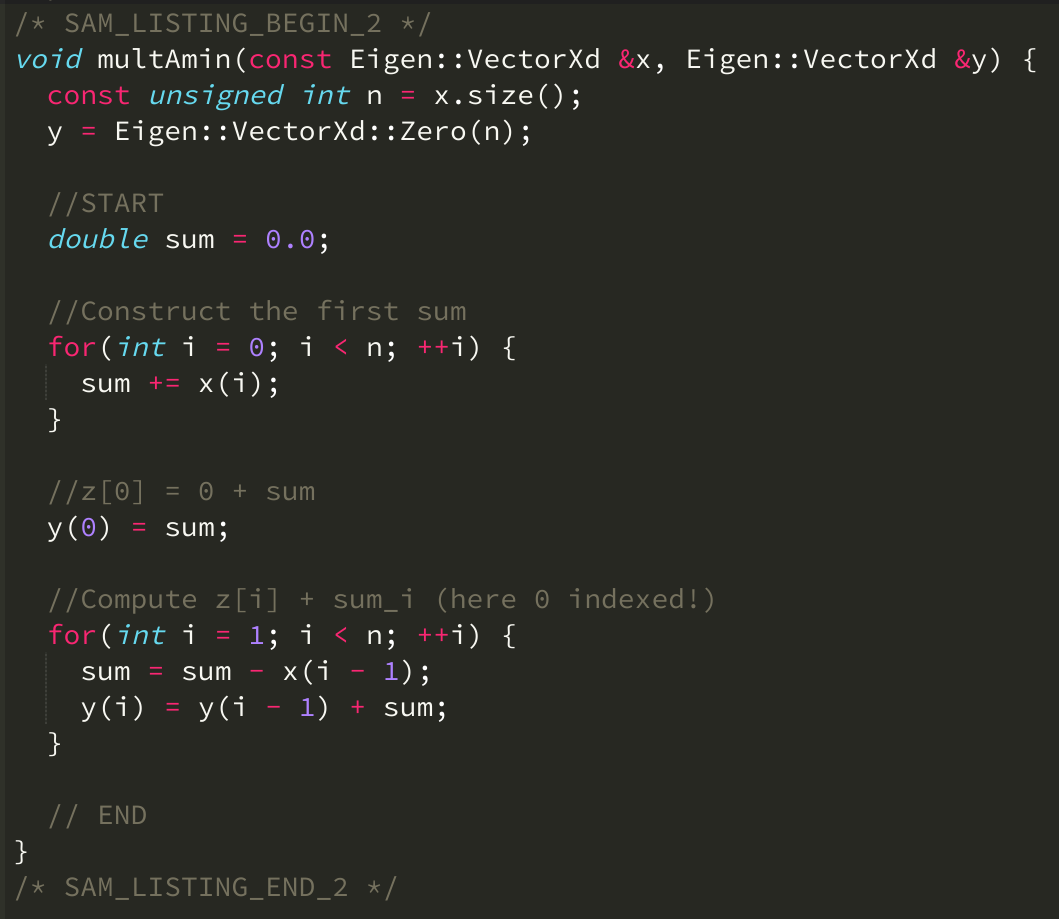
\includegraphics[width=0.8\linewidth]{1-7b.png}
\end{figure}

\subsection*{1-7.c}
As discussed above we get an asymptotic runtime complexity of $\mathcal{O}\left(n\right)$.

\subsection*{1-7.d}
We are tasked with comparing the results of both implementations using the class \verb|Timer|. We should report measurement in seconds with scientific notation using 3 decimal digits. This we can do using \verb|std::scientific| and \verb|std::setprecision(3)| we can add spacing using \verb|std::setw(15)|. We then construct a double loop structure as always looking something like the following piece of code.

\begin{lstlisting}[language=C++,
                   directivestyle={\color{black}}
                   emph={int,char,double,float,unsigned},
                   emphstyle={\color{blue}}
                  ]
for(int N = (1 << 5); N <= (1 << 12); N = N << 1) {
    for(int r = 0; r < nruns; ++r) {
        
    }
}
\end{lstlisting}
Where \verb|1 << 5 = 32| and $32 = 2^{5}$. We can then take timings by creating a new timer via \verb|Timer timer_name;| and start the timer via \verb|timer_name.start();| and stop the timer via \verb|timer_name.stop();|. We can then output the time using \verb|timer_name.min();| or \verb|timer_name.duration();|. The first one return the minimal time a loop took, as one can also take loop timinings with \verb|timer_name.loop();|. The second one returns the total amount the timer has been running, hence \verb|timer_name.min();| is more suitable here. The output will mostly be formatted something like the following code segment.

\begin{lstlisting}[language=C++,
                   directivestyle={\color{black}}
                   emph={int,char,double,float,unsigned},
                   emphstyle={\color{blue}}
                  ]
std::cout << std::setw(15) << N << std::scientific << std::setprecision(3)
          << std::setw(15) << tm_slow.min() << std::setw(15)
          << tm_fast.min() << std::endl;
\end{lstlisting}

\pagebreak

\subsection*{1-7.e}
We are given the following code segment.
\begin{figure}[!hbt]
    \centering
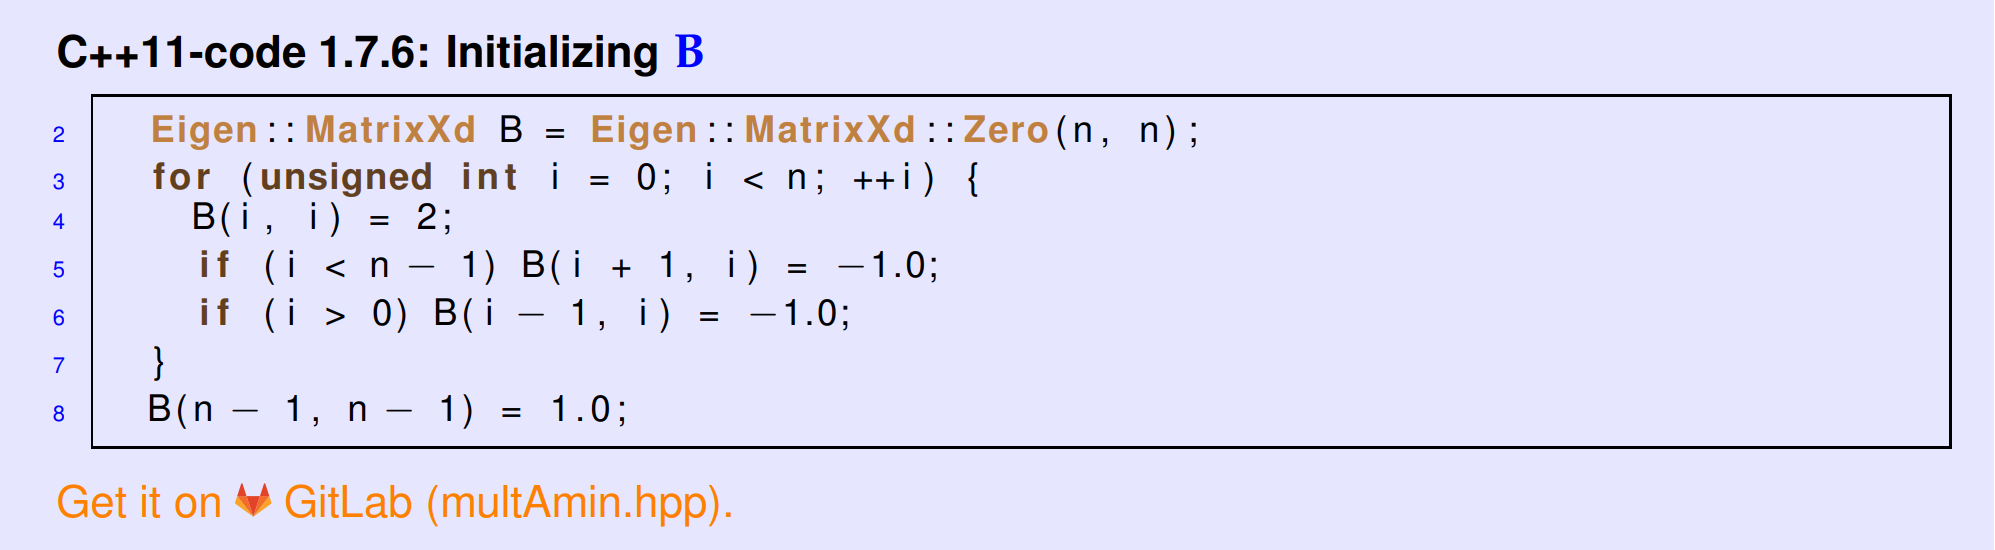
\includegraphics[width=1.0\linewidth]{1-7eCode.png}
\end{figure}

\noindent We are now tasked with sketching the matrix which is created here.  We can write this down as the following matrix definition.
\begin{equation*}
    \mathbf{B}_{i,j} = 
    \begin{cases}
        1 \quad &\text{if } i = j = n-1 \, ,\\
        2  &\text{if } i = j \neq n-1 \, ,\\
        -1 &\text{if } i = j - 1 \text{ or } i = j + 1 \, ,\\
        0 &\text{else.}
    \end{cases}
\end{equation*}
Which gives us the following matrix structure.
\begin{equation*}
    \begin{bmatrix}
        2 & -1 & 0 & 0 &\dots & 0 \\
        -1 & 2 & -1 & 0 & \dots & 0 \\
        0  & -1 & \ddots & \ddots & & \vdots \\
        \vdots & & \ddots & &-1 & 0\\
        & & &-1 &2 &-1\\
        0 & \dots & &0 & -1 & 1
    \end{bmatrix}
\end{equation*}
\subsection*{1-7.f} 
We are tasked to implement the function \verb|multABunitv()| where for $n=10$ we should compute $\mathbf{A}\mathbf{B}\mathbf{e}_{j}$ and $\mathbf{e}_{j}$ is the $j$-th unit vector in $\mathbb{R}^{n}$, $j = 1, \dots, n$ and return the result as the columns of a matrix in addition to printing the matrix. We now again need to consider the structure of the two matrices, because we have
\begin{equation*}
    \mathbf{A} = \begin{bmatrix}
        1 & 1 & 1 & \dots & 1 \\
        1 & 2 & 2 & \dots & 2 \\
        1 & 2 & 3 & \dots & 3 \\
        \vdots & \vdots & \vdots &\ddots & \vdots \\
        1 & 2 & 3 & \dots & n
    \end{bmatrix}
\end{equation*}
Let us first consider a small example for $n = 4$ and the first unit vector:
\begin{equation*}
    \mathbf{A} = \begin{bmatrix}
        1 & 1 & 1 & 1 \\
        1 & 2 & 2 & 2 \\
        1 & 2 & 3 & 3 \\
        1 & 2 & 3 & 4
    \end{bmatrix}
    *
    \begin{bmatrix}
        2 & -1 & 0 & 0 \\
        -1 & 2 & -1 & 0 \\
        0 & -1 & 2 & -1 \\
        0 & 0 & -1 & 1
    \end{bmatrix}
    *
    \begin{bmatrix}
        1 \\0 \\0 \\0
    \end{bmatrix}
    = 
    \begin{bmatrix}
        1 & 1 & 1 & 1 \\
        1 & 2 & 2 & 2 \\
        1 & 2 & 3 & 3 \\
        1 & 2 & 3 & 4
    \end{bmatrix}
    * \begin{bmatrix}
        2 \\ -1 \\ 0 \\ 0
    \end{bmatrix}
\end{equation*}
The matrix-vector product on the right can be computed using the function \verb|multAmin| we wrote in 1-7.b. The vector we multiply with is the $j$-th column of the matrix $\mathbf{B}$. We can hence use \verb|B.col(j)| to retrieve this. This results in the following code. 

\begin{figure}[!hbt]
    \centering
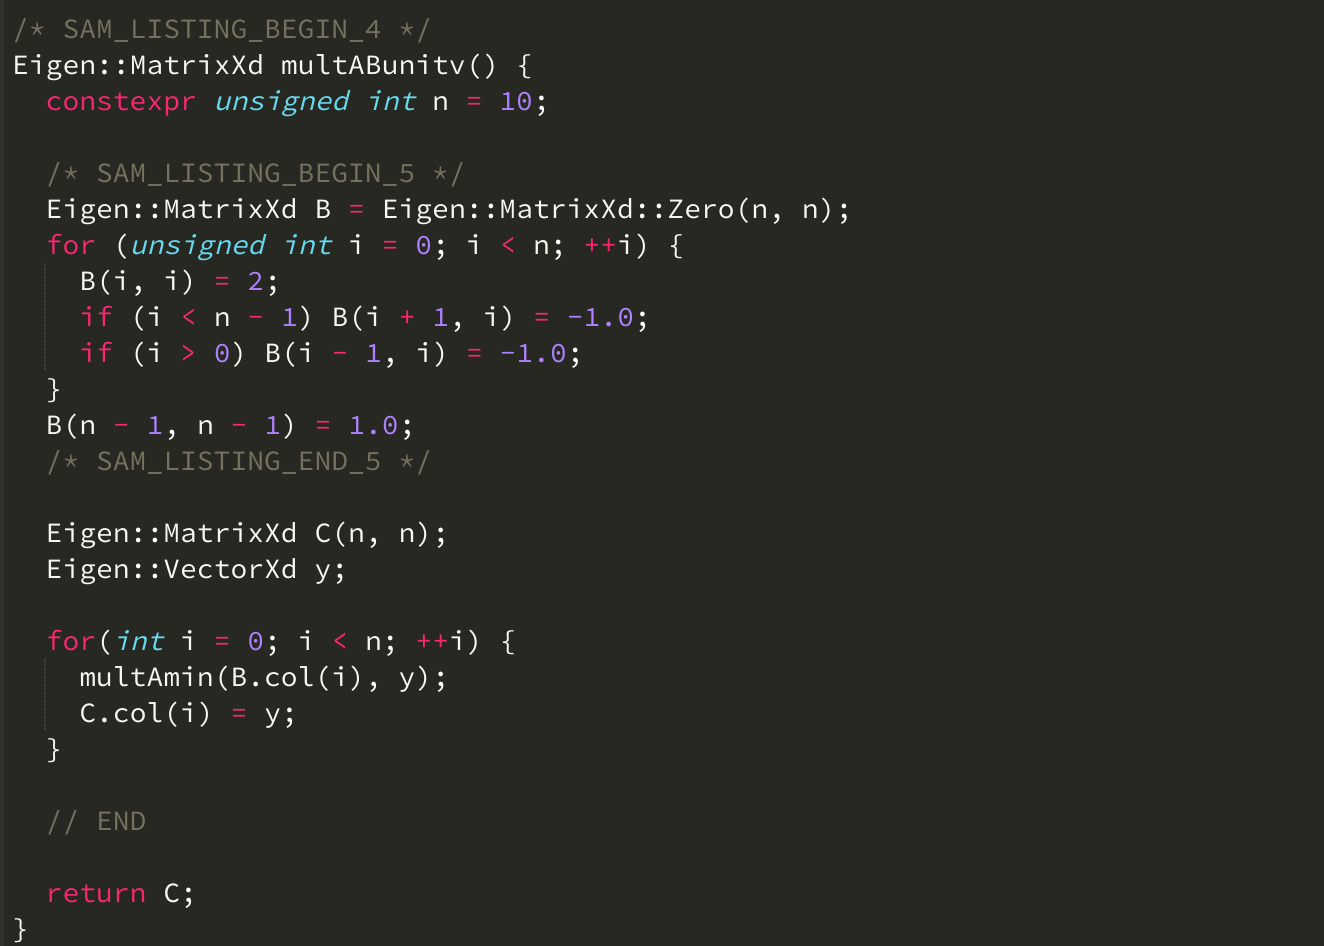
\includegraphics[width=1.0\linewidth]{1-7e.png}
\end{figure}

\end{document}
